\chapter{O InvestMVC}

O investidor interage apenas com o componente Orientado a Objetos, criando seu usuário e \textit{experts}, no qual serão persistidos. Além disso, o investidor também poderá ativar um \textit{expert}.

O componente Multiagentes vai verificar a tendência do Mercado de Moedas, por meio da plataforma MetaTrader. Sendo assim, o componente Multiagentes buscará na persistência o \textit{expert} que está ativo. Sabendo qual o \textit{expert} que foi ativado, o componente Multiagente faz a requisição de cálculos para os módulos C e Haskell. A partir desse resultado, o componente Multiagente procurará no Módulo Base de Conhecimento, a alavancagem (quanto deve arriscar) e os valores de entrada para o método de Correlação de Pearson, Fibonacci e Mínimos Quadrados. Caso todas as especificações para o componente Multiagente sejam obedecidas, ele informa ao componente MQL para realizar uma compra ou venda.

\begin{figure}[H]
\centering
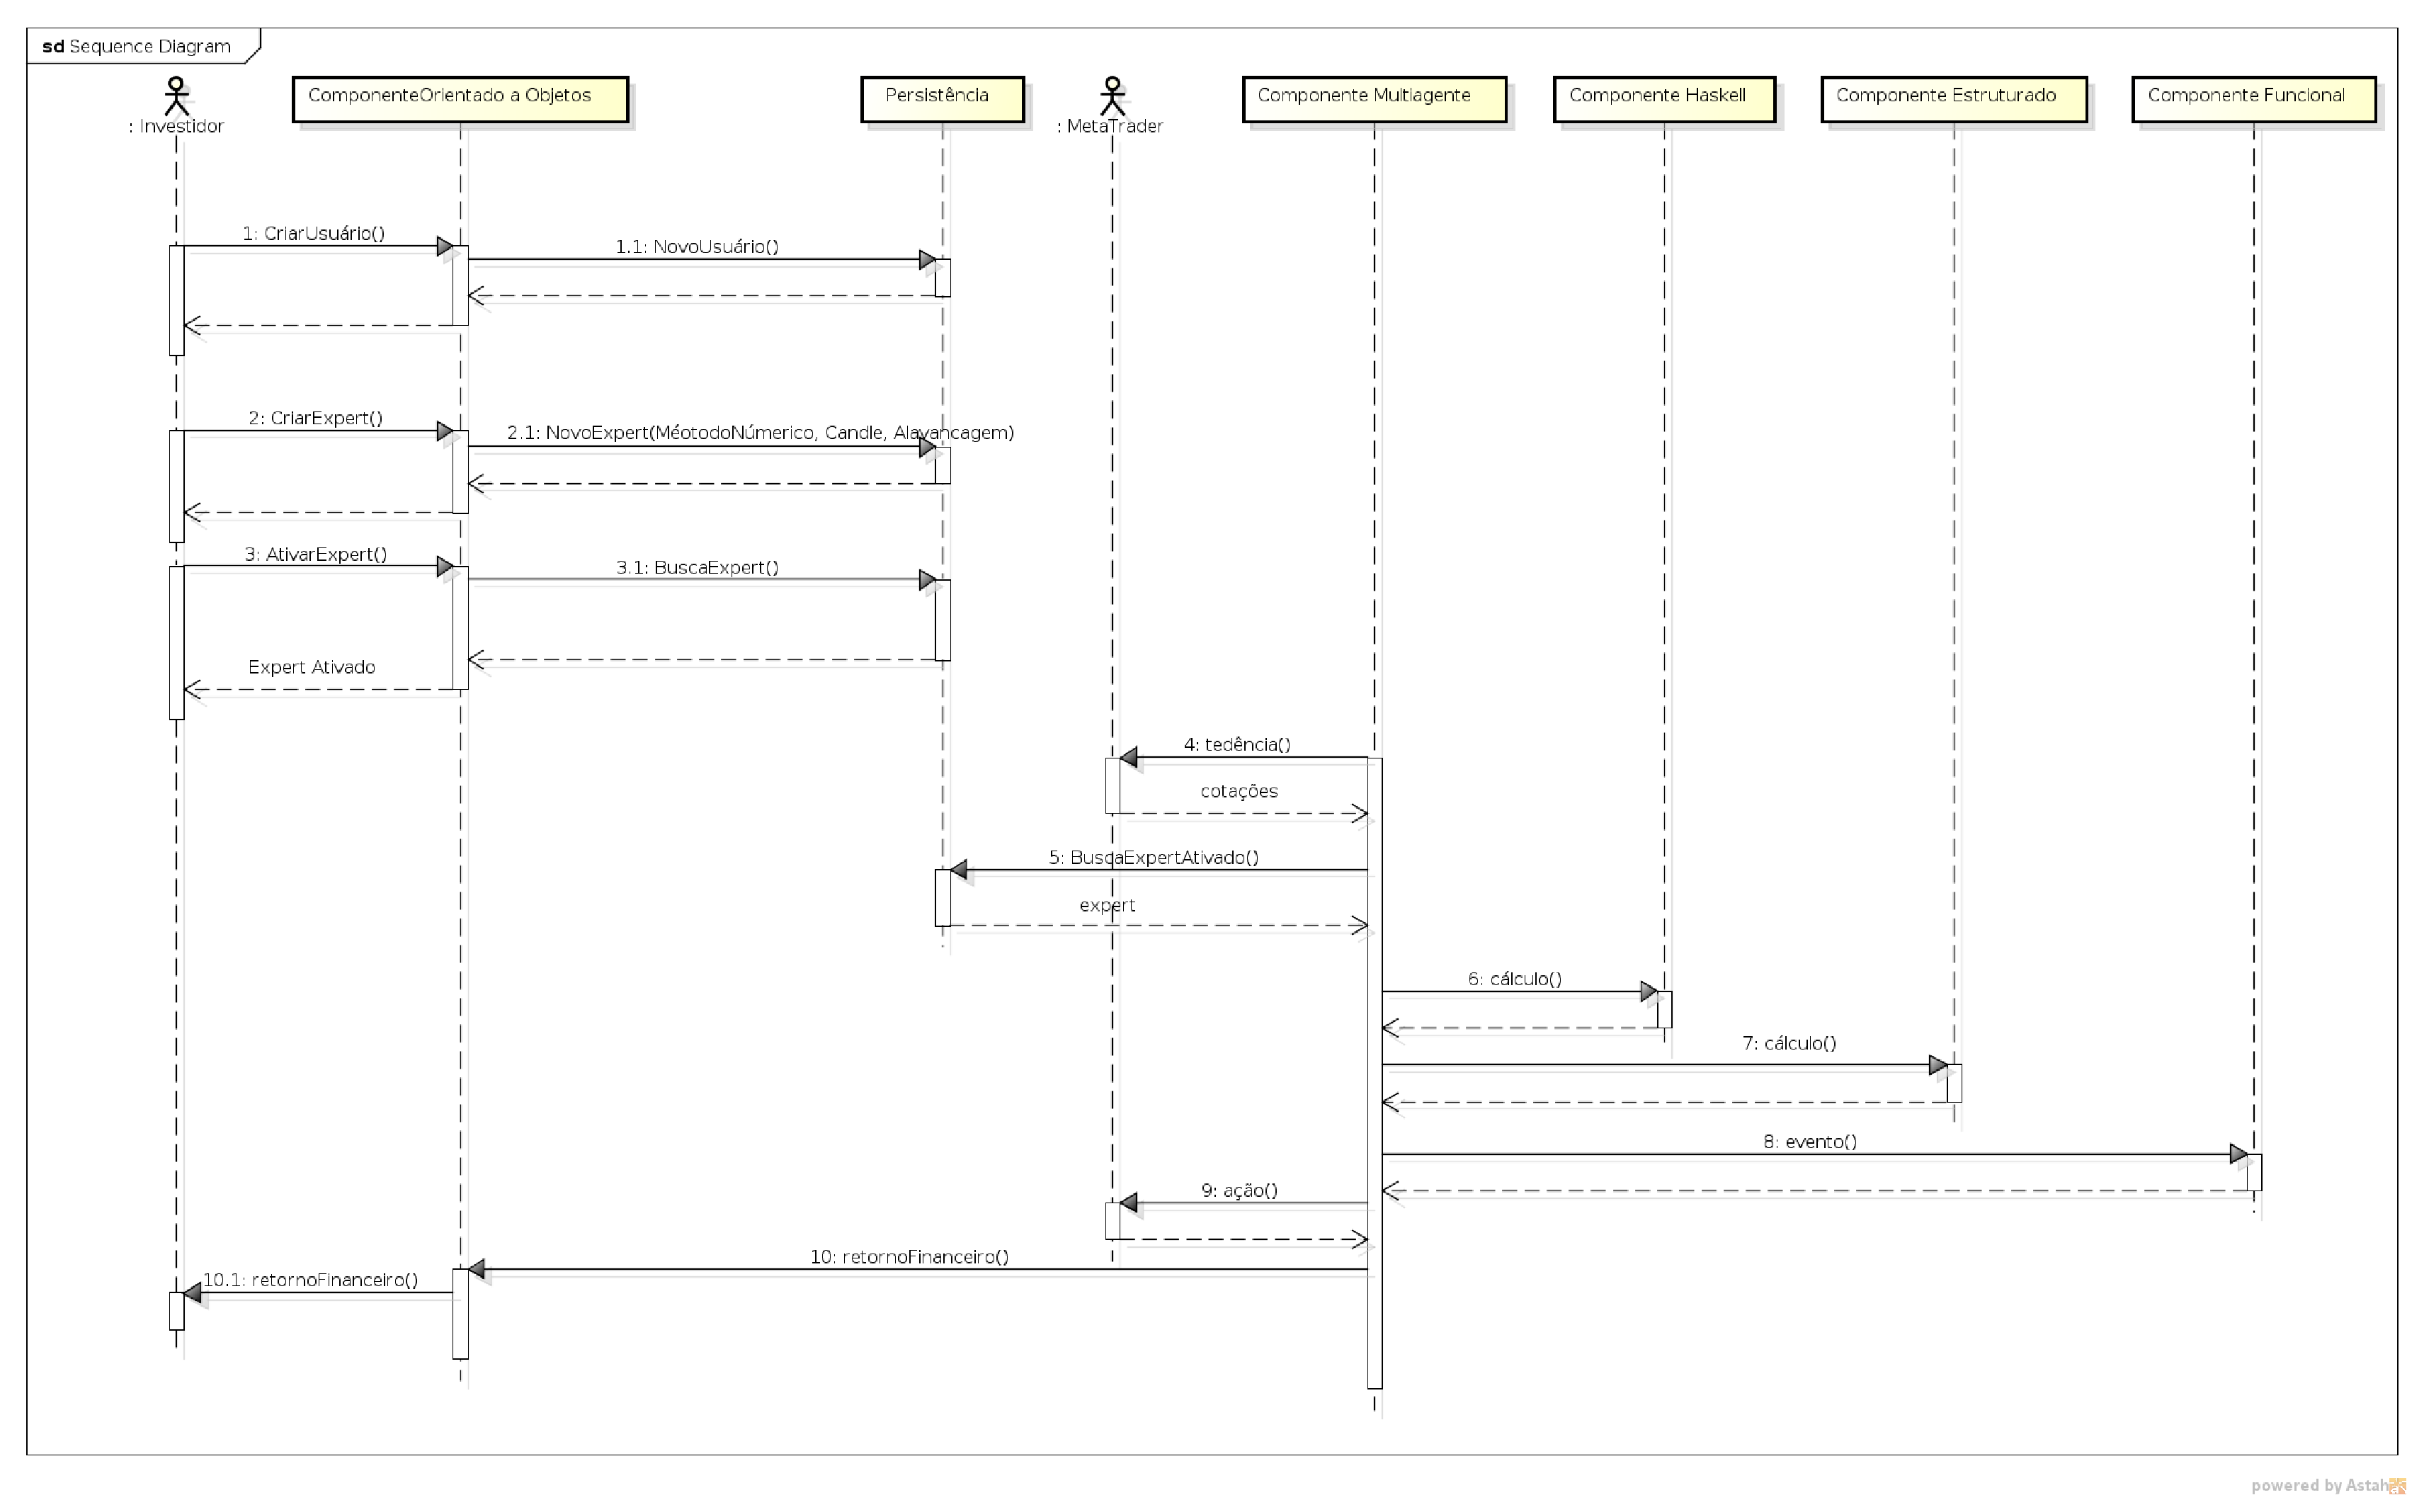
\includegraphics[width=0.9\textwidth]{figuras/sequencia}
\caption{Diagrama de Sequência InvestMVC} 
\label{sequencia}
\end{figure}
